\documentclass[tikz,border=10pt]{standalone}
\usepackage{amsmath,amssymb}
\usetikzlibrary{arrows.meta,positioning,calc}

\definecolor{nodecol}{RGB}{40,40,160}
\definecolor{edgecol}{RGB}{110,100,200}
\definecolor{topicc}{RGB}{210,90,20}
\definecolor{userc}{RGB}{0,130,90}    % positive sample
\definecolor{negc}{RGB}{180,40,40}    % negative samples

\tikzset{
  neuron/.style={circle, draw=nodecol, thick, minimum size=0.85cm, inner sep=0pt, font=\small},
  active/.style={neuron, draw=topicc, fill=topicc!15},
  conn/.style={edgecol!35, line width=0.3pt},
  lbl/.style={font=\bfseries\small, text=black!70, align=center},
}

% \sgnsstep{y-shift}{step id}{active input (1-3)}{pos user}{neg1}{neg2}{neg3}{logits p/n1/n2/n3}{topic id}
\newcommand{\sgnsstep}[9]{%
\begin{scope}[shift={(0,#1)}]
  % ---- pair box ----
  \node[draw=black!60, rounded corners=3pt, inner sep=5pt, anchor=west, align=left,
        text width=4.3cm, font=\small] (s#2box) at (-6.3,0)
    {\textbf{Step #2}\\[2pt]
     \textcolor{userc}{positive: $(t_{#9},u_{#4})$}\\[2pt]
     \textcolor{negc}{negatives:}\\
     \textcolor{negc}{$(t_{#9},u_{#5})$, $(t_{#9},u_{#6})$,}\\
     \textcolor{negc}{$(t_{#9},u_{#7})$}};

  % ---- input layer (one-hot) ----
  \foreach \i/\y in {1/1.1, 2/0.0, 3/-1.1}{
    \ifnum\i=#3 \def\sty{active}\else\def\sty{neuron}\fi
    \node[\sty] (s#2i\i) at (0,\y) {\ifnum\i=#3 1\else 0\fi};
  }
  \node at (0,1.75)  {$\vdots$};
  \node at (0,-1.75) {$\vdots$};
  \node[left=3pt of s#2i#3, font=\small, text=topicc] (s#2tl) {$t_{#9}$};
  \draw[->, thick, black!60] (s#2box.east) -- (s#2tl.west);

  % ---- hidden layer = topic embedding ----
  \node[neuron] (s#2h1) at (3.4, 0.85) {\ifcase#3\or 1.9\or 6.3\or -2.8\fi};
  \node at (3.4,0) {$\vdots$};
  \node[neuron] (s#2h2) at (3.4,-0.85) {\ifcase#3\or -0.7\or 0.2\or 3.5\fi};

  % ---- edges input -> hidden (active topic selects its weights) ----
  \foreach \i in {1,2,3}{\foreach \h in {1,2}{
    \ifnum\i=#3 \draw[topicc, line width=1pt] (s#2i\i) -- (s#2h\h);
    \else \draw[conn] (s#2i\i) -- (s#2h\h);\fi
  }}

  % ---- output layer: 1 positive + 3 negative users ----
  \foreach \a/\b/\c/\d in {#8}{
    \foreach \k/\y/\lg/\col/\tgt/\txt in {
        1/1.65/\a/userc/1/Positive,
        2/0.55/\b/negc/0/Negative,
        3/-0.55/\c/negc/0/Negative,
        4/-1.65/\d/negc/0/Negative}{
      \node[neuron, draw=\col, fill=\col!10] (s#2o\k) at (6.8,\y) {\lg};
      \pgfmathsetmacro\sv{1/(1+exp(-(\lg)))}
      \draw[-{Stealth[length=2mm]}, thick, \col] (s#2o\k.east) -- ++(0.8,0)
          node[right, font=\small] {$\sigma\!\rightarrow\!\pgfmathprintnumber[fixed,precision=2]{\sv}$};
      \node[anchor=west, font=\small, text=\col] at (9.9,\y) {\tgt\ \ \txt};
    }
  }
  \foreach \h in {1,2}{\foreach \oo/\col in {1/userc,2/negc,3/negc,4/negc}{
    \draw[\col!65, line width=0.8pt] (s#2h\h) -- (s#2o\oo);
  }}
  \node at (6.8,-2.3) {$\vdots$};
  \node[anchor=west, font=\scriptsize, text=black!50] at (7.1,-2.3)
      {remaining users: not computed};
\end{scope}}

\begin{document}
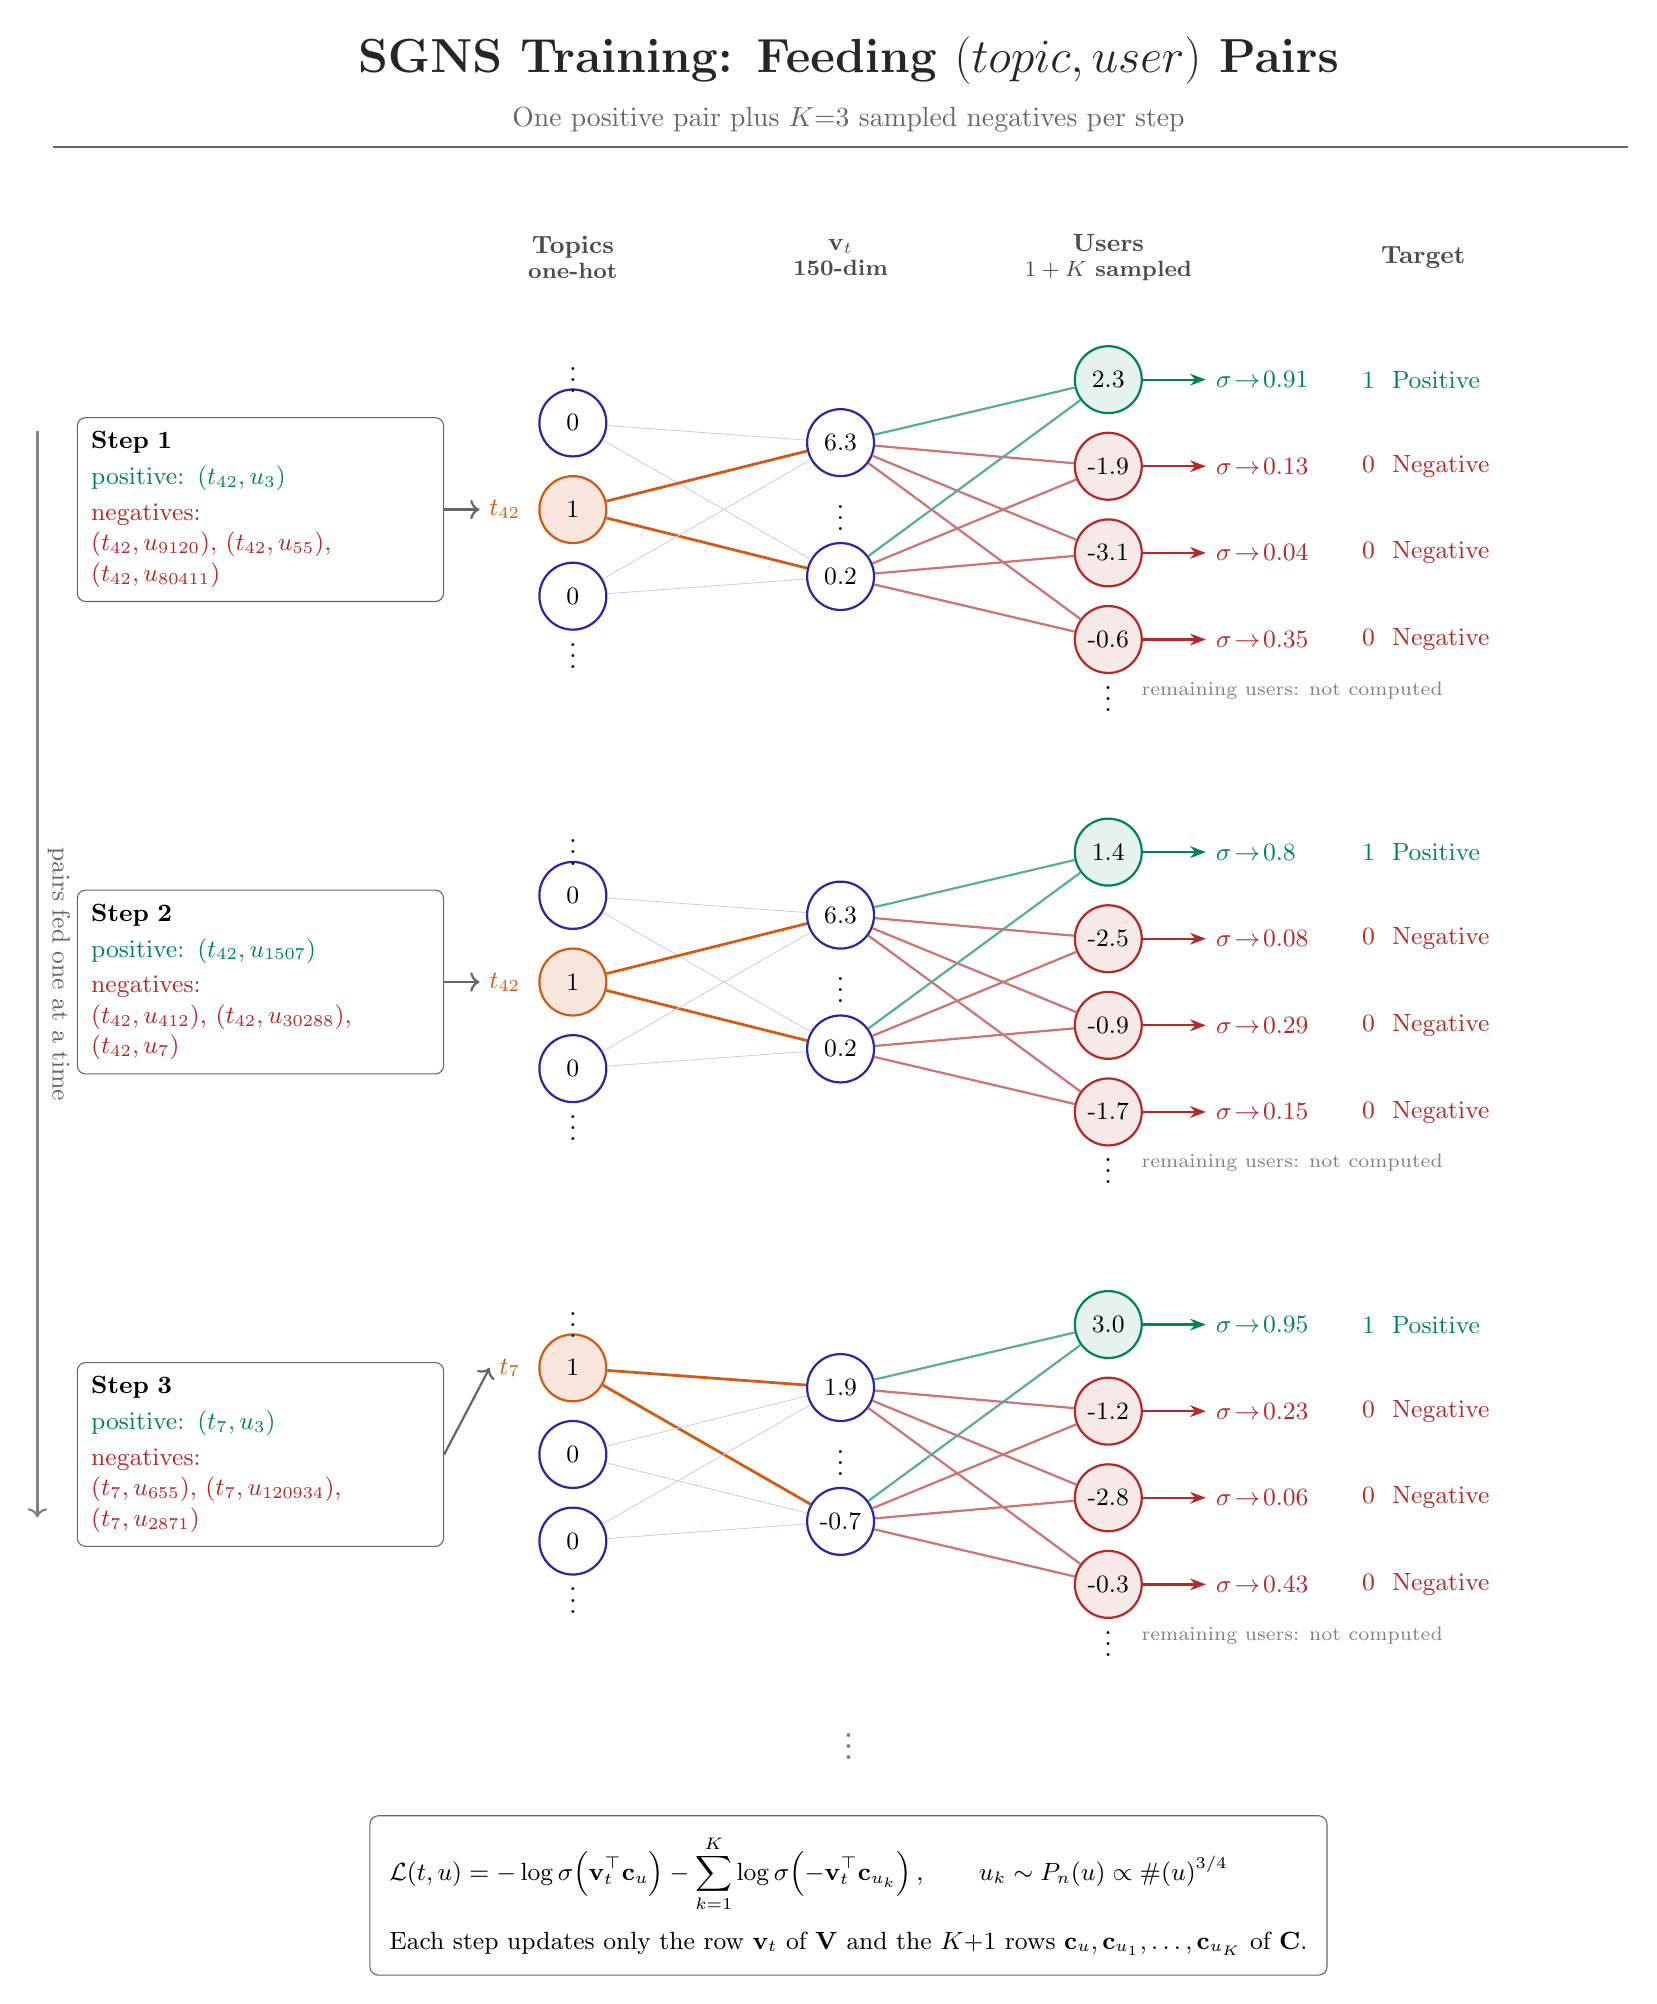
\begin{tikzpicture}

% ---------- Title ----------
\node[font=\LARGE\bfseries, text=black!85] (title) at (3.5,5.7)
  {SGNS Training: Feeding $(topic,user)$ Pairs};
\node[font=\normalsize, text=black!60, below=1pt of title]
  {One positive pair plus $K{=}3$ sampled negatives per step};
\draw[black!60, line width=0.8pt] (-6.6,4.6) -- (13.4,4.6);

% ---------- Column headers ----------
\node[lbl] at (0,3.2)   {Topics\\[-2pt]\footnotesize one-hot};
\node[lbl] at (3.4,3.2) {$\mathbf{v}_t$\\[-2pt]\footnotesize 150-dim};
\node[lbl] at (6.8,3.2) {Users\\[-2pt]\footnotesize $1+K$ sampled};
\node[lbl] at (10.8,3.2) {Target};

% ---------- Three consecutive training steps ----------
\sgnsstep{0}{1}{2}{3}{9120}{55}{80411}{2.3/-1.9/-3.1/-0.6}{42}
\sgnsstep{-6}{2}{2}{1507}{412}{30288}{7}{1.4/-2.5/-0.9/-1.7}{42}
\sgnsstep{-12}{3}{1}{3}{655}{120934}{2871}{3.0/-1.2/-2.8/-0.3}{7}

% time arrow
\draw[->, thick, black!50] (-6.8,1.0) -- (-6.8,-12.8)
  node[midway, sloped, above, font=\small, text=black!60] {pairs fed one at a time};
\node[font=\Large, text=black!50] at (3.5,-15.6) {$\vdots$};

% ---------- Loss / update summary ----------
\node[draw=black!60, rounded corners=3pt, inner sep=7pt, align=left, font=\small]
  at (3.5,-17.6)
  {$\displaystyle \mathcal{L}(t,u)=-\log\sigma\!\left(\mathbf{v}_t^{\top}\mathbf{c}_u\right)
     -\sum_{k=1}^{K}\log\sigma\!\left(-\mathbf{v}_t^{\top}\mathbf{c}_{u_k}\right),
     \qquad u_k\sim P_n(u)\propto \#(u)^{3/4}$\\[6pt]
   Each step updates only the row $\mathbf{v}_t$ of $\mathbf{V}$ and the $K{+}1$ rows
   $\mathbf{c}_u,\mathbf{c}_{u_1},\dots,\mathbf{c}_{u_K}$ of $\mathbf{C}$.};

\end{tikzpicture}
\end{document}
